\chapter{Back-end Implementation}\label{ch:4}

The following sections will present the implementation of our tool in more detail.
It will cover the relational schema chosen for storing the repository information in the database, the mining algorithm with which the application retrieves the repository data from the GitHub API and repository web-pages and, lastly, the components that make up the architecture of the application.

\section{Relational Schema}

In order to design the relational schema for the database, we first have to pose the question: \emph{Which information is relevant to select software repositories for MSR studies?}
Although the introduction only briefly skimmed over some examples of useful data, there are many other characteristics based on which researchers may want to limit their selection.
The following is a list of all the data that we have chosen to mine for repositories, as well as explanations on why said data may be valuable to researchers:
\begin{itemize}
    \item \textit{The full repository name, formatted as:} \code{user_name/repo_name}
    \\The identifier of a repository. While multiple repositories from different owners can have the same name (which makes sense to accommodate forks), a single user cannot create multiple repositories with the same name..
    \item \textit{An indication as to whether a project is a fork of an existing project.}
    \\Forking is central to the Git ecosystem. However in some cases, researchers may want to exclude forks when sampling, as they contain little to no modifications made to the forked project. Due to how easily they can be created, ``forks with no changes'' may not harbor any useful information to a study, and only serve to bloat a dataset~\cite{FORKS}. On the other hand, researchers may also want to limit the study to only forks of a popular project, with the goal of observing which features of the forked projects may have changed across various forks or, more in general, to answer specific research questions about forks.
    \item \textit{The number of commits.}
    \\The number of commits is by far the most commonly observed attribute for determining the scope of a project, as they equate to checkpoints in development. It is very common for inactive or small personal projects (which comprises the majority of projects on GitHub~\cite{COMMITS}) to have a low number of commits.
    \item \textit{The number of branches.}
    \\Branches represent several lines in development of a software project~\cite{GIT}. They too are good indicators of project scope, as more serious projects generally use more than the single default branch.
    \item \textit{The number of releases.}
    \\Releases are GitHub's method of packaging and providing software to users~\cite{GITHUBHELP}. Such a selection criterion is particularly useful for studies focusing on release-level analysis (e.g., on automatically generating release notes).
    \item \textit{The number of contributors.}
    \\As the name suggests, project contributors are GitHub users who have contributed to a project, albeit not as part of the core development team~\cite{GITHUBHELP}. A high contributor count in a public repository is a good indication of how much the community is engaged in a project. It should be of no surprise that personal projects tend not to have high contributor counts.
    \item \textit{The number of watchers.}
    \\The watchers of a public repository are users who have asked to be notified of activity in a repository, but have not become collaborators~\cite{METRICSWATCHERS}. Watchers can be interpreted as an extension to contributors. Although not contributing to projects in a direct way, they tend to be engaged in the discussions surrounding its development, some even going so far as to becoming future contributors~\cite{WATCHERS14}.
    \item \textit{The number of stars.}
    \\Stars were introduced in 2012 as an alternative way of keeping track of interesting projects without receiving notifications~\cite{STARS}. In essence, a project's star count is attributed to its notoriety on the platform. Given how the default sorting order for both the Advanced Search and API is by stars, projects with higher star counts appear first in searches, making them more popular.
    \item \textit{Project size}
    \\A lot of the aforementioned project characteristics were linked to the symbolic size of the project: how well-known it is within the community, and how much the community cares about it. It is also as important to take the literal size of a project, as in the amount of physical space its files take up.
    \item \textit{Date of creation, last update, last commit and last push}
    \\Filtering by created date allows researchers to focus exclusively on repositories from a restricted time frame, while dates such as the date of last update or commit provide a good indication into whether a project is still active, or if it has been abandoned.
    \item \textit{The total set of programming languages in a project}
    \\As important as the predominant language is, some studies may also require a complete overview of all languages present in a project.
    \item \textit{The main programming language of a project.}
    \\While repositories tend to house a variety of files written in different languages, a project usually tends to have the majority of its files written in a specific language. Such a language with the highest degree of presence in a project is ofter referred to as the \textit{main language} of that project. Some studies, such as those focusing on correlating the language of a project with its code quality~\cite{QUALITY}, are dependent on the ability to filter projects based on the predominant language.
    \item \textit{The number of issues: both open and total}
    \\Issues are community-launched and collaborator-moderated discussion threads, aimed at addressing project limitations and suggesting changes~\cite{GITHUBHELP}. Studies centered on analysing issues, such as those analysing issue comments~\cite{ISSUES}, require selecting repositories that have either open or closed issues.
    \item \textit{The number of pull requests: both open and total}
    \\Pull requests are changes proposed to a repository by project contributors, which through their dedicated discussion threads, are either accepted or rejected by the core development team~\cite{GITHUBHELP}. Studies focusing on analysing aspects of pulls, such as those analysing the characteristics of accepted and rejected pull requests~\cite{PULLS}, require a sample of repositories that have them.
    \item \textit{The project labels}
    \\Labels are descriptive tags assigned to issues and pull requests for classification purposes~\cite{LABELS}. Filtering repositories by the labels they use allow the researcher to focus on specific development activities, such as code refactoring and documentation issues.
    \item \textit{Project license}
    \\While on the surface mining the licensing information of a project makes sense for bookkeeping purposes, said data may be of use to researchers as well. Several studies were conducted with respect to repository licensing, examples include the effect of licensing bugs on the projects that use them~\cite{LICENSEBUGS}, along with how certain license usage and changes in one project effects other projects depending on them~\cite{LICENSECHANGE}.
    \item \textit{Whether the project is archived}
    \\Project archiving was introduced as a means of signalling to users that the project is discontinued and that it is no longer maintained by its authors and collaborators~\cite{ARCHIVINGREPOS}. Researchers can use this information to filter out inactive projects from samples they wish to study.
    \item \textit{Whether the project has a wiki}
    \\Wikis are pages dedicated to hosting the documentation of a project~\cite{WIKIS}. The presence of a wiki may indicate that a project is well documented. While this can be an indication, it is not a guarantee, since some wikis may just be empty.
\end{itemize}

\noindent
Although not subject to many studies, the following information is useful for bookkeeping:

\begin{itemize}
    \item \textit{The name of the default project branch}
    \item \textit{The external project homepage}
    \item \textit{The secure hash algorithm (SHA) hash of the last commit}
\end{itemize}

\newpage

\noindent
Having outlined the information relevant to a repository, the following schema (shown in Figure~\ref{fig:1}) has been constructed for the database:

\begin{itemize}
    \item \code{repo}
    \\Table dedicated to storing all the statistical information (excluding the labels and languages) related to a repository. This includes everything from the repository \code{name}, whether the repository is a fork of an existing repository (\code{is_fork}), whether the repository \code{is_archived}, whether its wiki is enabled (\code{has_wiki}), the \code{main_language} of a repository, the name of the \code{default_branch}, the assigned repository \code{license}, the external project \code{homepage}, the \code{size} of the repository in bytes, the date of creation, last update, last commit and last push (\code{created_at}, \code{updated_at}, \code{committed_at} and \code{pushed_at} respectively), the number of \code{branches}, \code{releases}, \code{contributors}, \code{watchers}, \code{stargazers}, \code{forks}, \code{total_issues}, \code{open_issues}, \code{total_pull_requests} and \code{open_pull_requests}.
    \item \code{repo_language}
    \\Given that each repository can have anywhere between no languages (in the case of empty repositories) and many languages, it was necessary to separate repository languages into a dedicated table, and link it to the repository table via a many-to-one relationship. Each row of this table stores a reference to a repository (\code{repo_id}), the name of the language that repository uses (\code{repo_language_name}), and the cumulative file size in bytes for that particular language (\code{size_of_code}).
    \\Keep in mind that the \code{main_language} of a repository is also present in this table. While \code{repo} only keeps the name of the \code{main_language}, \code{repo_label} also stores the size the language takes up.
    \item \code{repo_label}
    \\As is the case with languages, a repository can have many labels, or no labels at all. Each row of this table stores a reference to a repository (\code{repo_id}) and the name of the label said repository uses (\code{repo_label_name}).
    \item \code{access_token}
    \\Table dedicated to storing the access tokens for the miner, which are required to use the GitHub API\@. The original idea was to use multiple tokens during mining, and switch out tokens whenever their request rate limit was exceeded. This idea was scrapped due to GitHub easily detecting when multiple tokens were associated to an IP address, and suspending the accounts linked to these tokens.
    \item \code{supported_language}
    \\Responsible for storing the languages which will be mined by the application.
    \item \code{crawl_job}
    \\Responsible for keeping track of the mining progress for each of the supported languages. Every \code{crawl_job} is mapped to exactly one \code{supported_language}. The \code{crawled} column stores the lower bound of the date and time interval up to which the repositories have been mined for a language, while the upper bound of the interval is the beginning of 2008\footnote{The start of the year during which GitHub was founded was chosen as the lower bound for repository mining.}. If there is no entry for a specific language, then no repositories have been mined for that language.
\end{itemize}

Note that the \code{crawled} column of \code{repo}, \code{repo_label} and \code{repo_language}, as well as the \code{added} column of \code{access_token} and \code{supported_language} were only used for debugging purposes, and represent the date and time at which the database records were created.

\begin{figure}[h!]
    \centering
    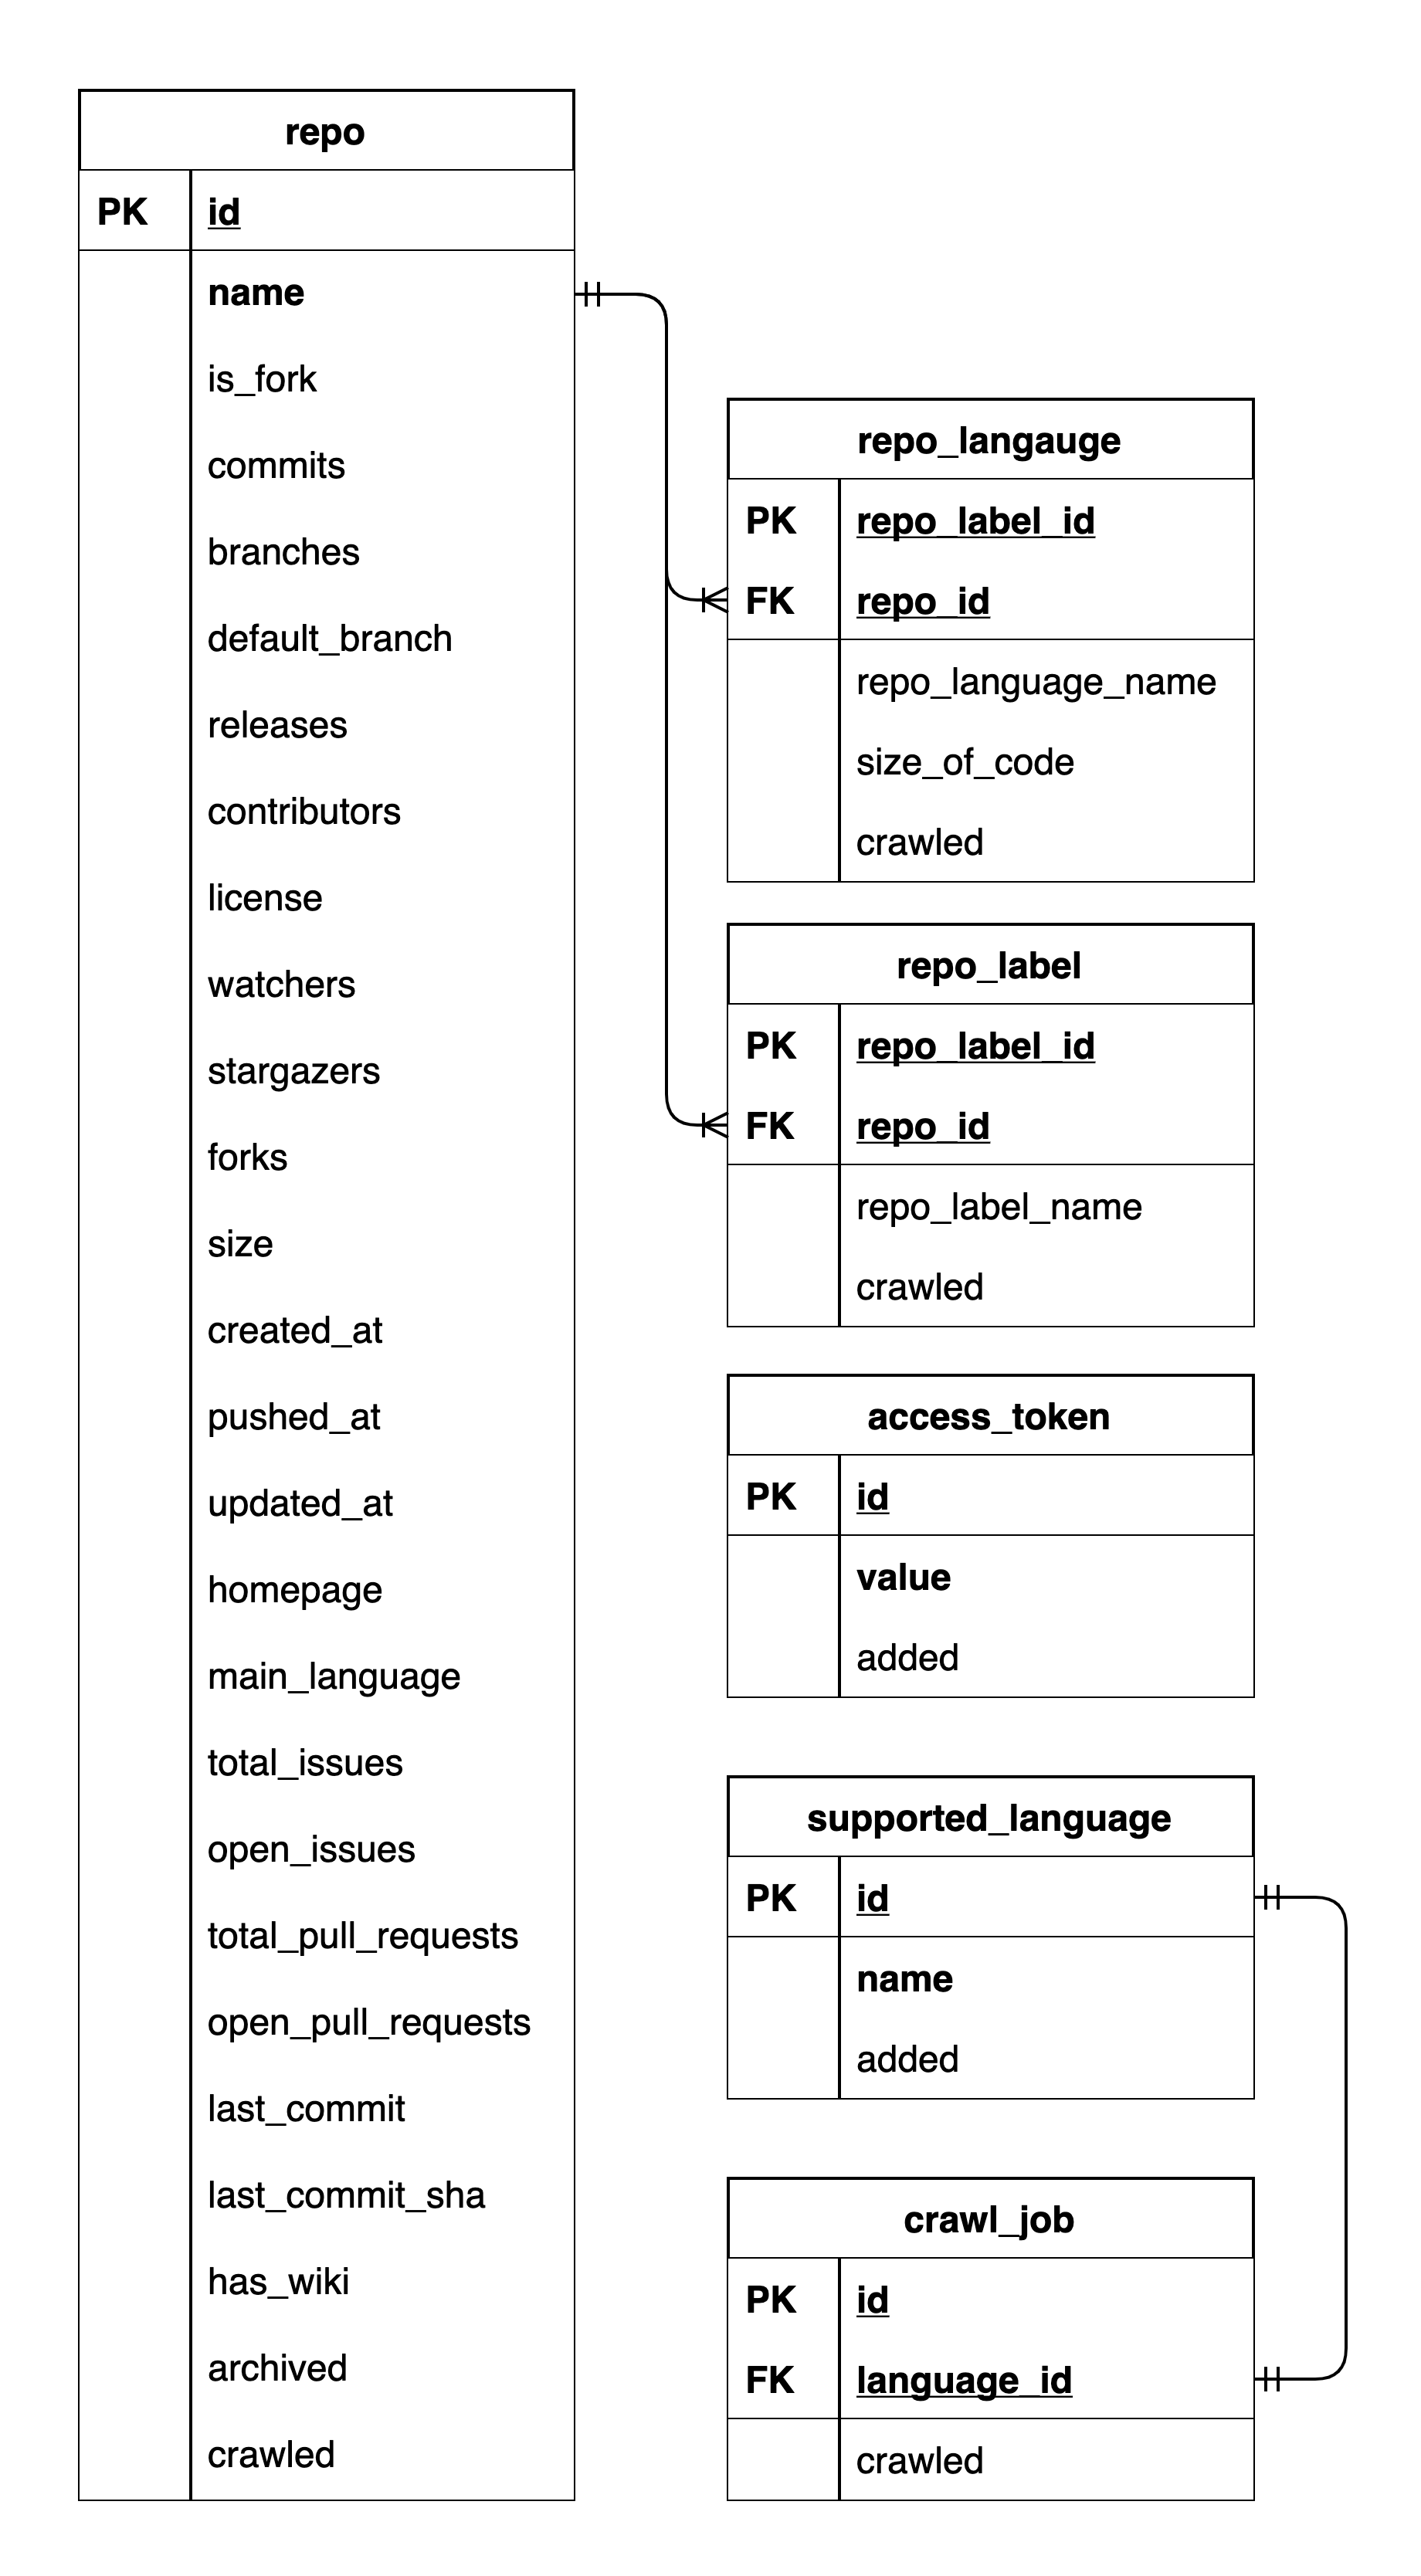
\includegraphics[width=0.7\linewidth]{relational}
    \caption[Relational database schema]{The relational schema of the database.}
    \label{fig:1}
\end{figure}

\newpage
\section{The Mining Algorithm}

The mining algorithm is the core of our search engine.
In broad terms, the miner is responsible for mining all the public projects written in certain languages, from oldest to newest created.
It is important to note that the miner currently prioritises repositories consisting predominantly of code written in more popular languages, which include: Java, Kotlin, C, C++, Python, JavaScript and TypeScript.
Since mining is sequentially performed for each language, all the repositories of one language have to be mined before moving to the next one.
The mining algorithm works as follows:

The application retrieves the list of all supported languages from the \code{supported_language} table.
For each language, the application then checks if any prior mining has been conducted for said language, by looking at its associated record in the \code{crawl_job} table.
If no prior mining was conducted for the language, the application mines all repositories created between January 1st 2008 and two hours before the mining process was started\footnote{Due to the fact that it takes time for GitHub's internal database to sync newly created projects, its best to avoid mining anything created within the past 2 hours.}.
Conversely, the mining is resumed from the date indicated in the database, and the application mines all repositories created and updated\footnote{The reason as to why we need to mine repositories updated in that time frame, is to account for any changes to records already existing in the application database.} between that date and two hours before the mining process was started.

Having selected a time interval for mining a language, there may be more repositories than can be retrieved by the GitHub API\@.
To work around this issue, if a time interval has too many results, then we split it into more manageable chunks.
Interval mining is performed in the following manner:
\begin{enumerate}
    \item A ``request stack'' is defined, used for storing future mining intervals. The first element of the data structure will always be the broad mining interval of a language, described previously in more detail.
    \item We take a date interval from the top of the stack. Said interval is passed to a GitHub API call, requesting all projects and associated forks of a certain language created during that time. If the stack is empty, then the crawl is finished.
    \item Depending on the number of total results returned in the response:
    \begin{enumerate}
        \item If the number of results is greater than 1000, then the time interval is split in half, and the two new intervals are pushed to the stack\footnote{In order to ensure that the newly obtained intervals are sequentially traversed, the second interval is pushed first followed by the first interval.}. Go back to 2.
        \item Otherwise, we iterate over the result list. For each result:
        \begin{enumerate}
            \item Scrape the missing information from the repository web-page, and save the full record to the database.
            \item Using the GitHub API, retrieve the repository labels, and save them to the
            \\database.
            \item Using the GitHub API, retrieve the repository languages, and save them to the database.
        \end{enumerate}
        \item After iterating through all the results, go back to 2.
    \end{enumerate}
\end{enumerate}

\newpage
\section{Application Architecture}

This following section will explore the architecture of the application server, as well as how each of the components interact to create a cohesive system.
A full overview of the system can be seen in Figure~\ref{fig:2}.
Since the previous sections were exclusively dedicated to the mining algorithm and database structure, there is not much need to talk about their components.
The following sections will however focus on the GitHub API Service, GitHub Web-page Crawler Service, Database Services and the REST Controllers.

\begin{figure}[h!]
    \centering
    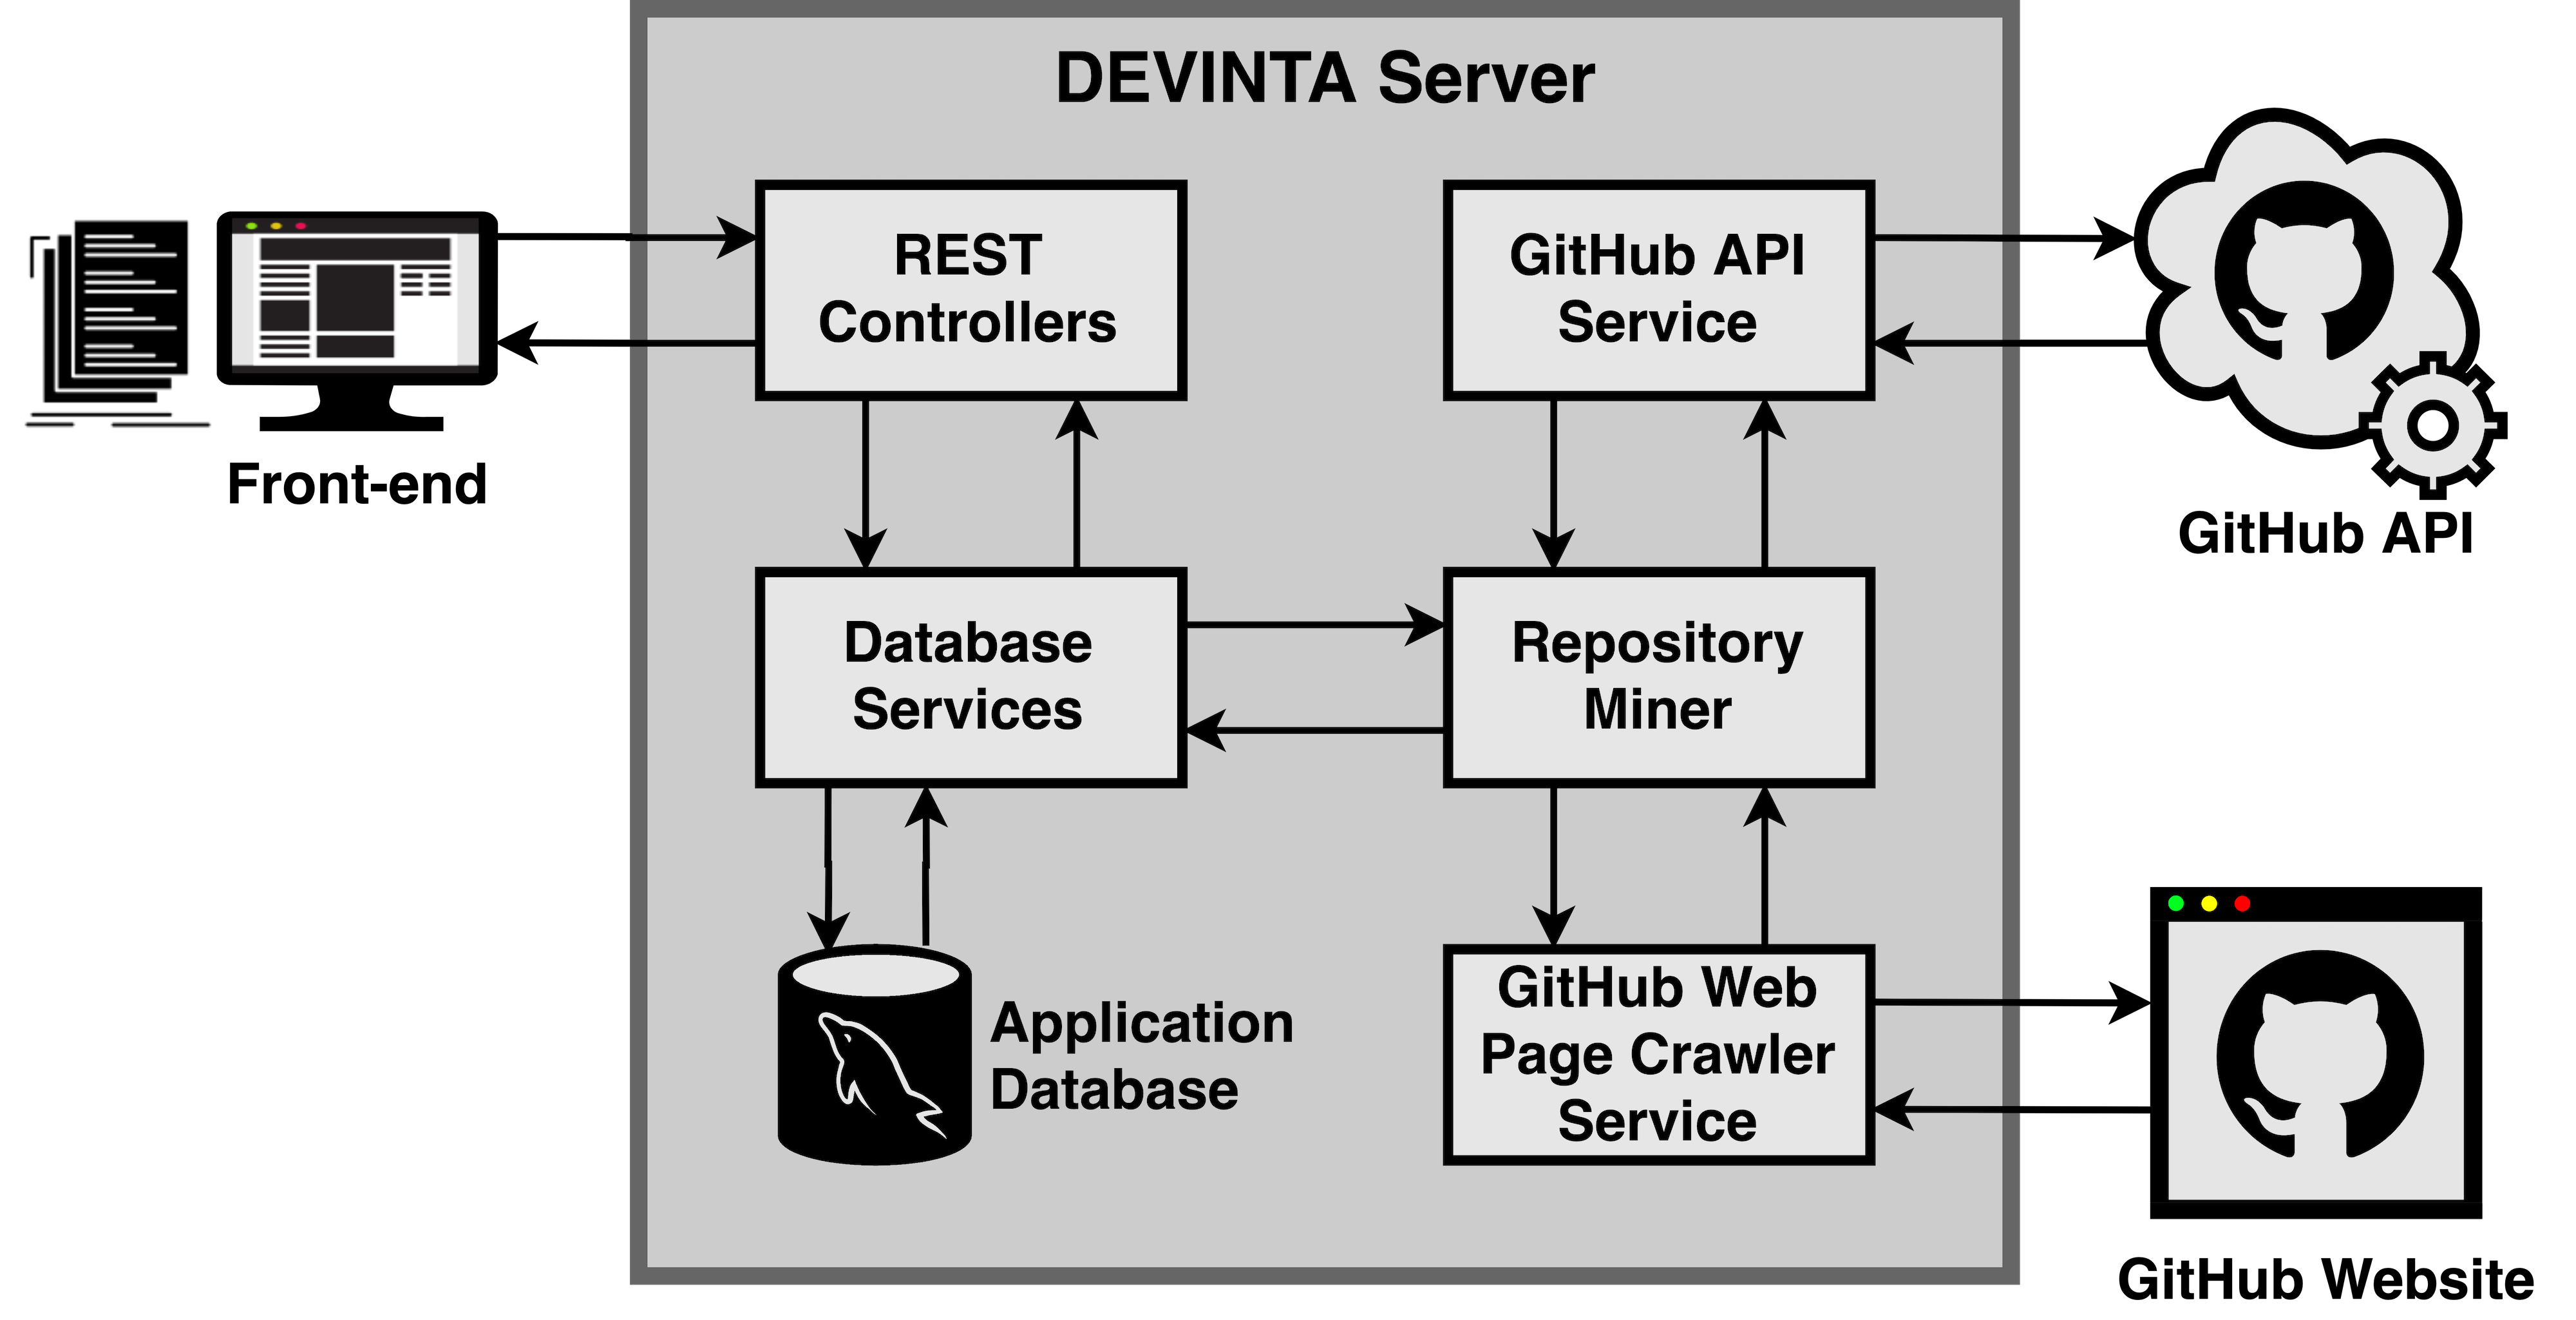
\includegraphics[width=1\linewidth]{architecture}
    \caption[Application architecture]{The application architecture.}
    \label{fig:2}
\end{figure}

\subsection{GitHub API Service}

The API Service is a component dedicated entirely to making REST requests to the GitHub Core and Search APIs.
It is exclusively used by the miner, which provides it with mining-specific arguments, such as time intervals to mine, the name of the language whose repositories we wish to mine, and the access tokens required to authenticate the requests.
All of the aforementioned requests are performed through a single OkHttp Client instance, created on application startup.
Obtained responses are passed directly back to the miner for further processing, decision-making and storage.
Supported methods of the GitHub API layer include:
\begin{enumerate}
    \item Verifying if an access token has not exceeded its request limit;
    \item Retrieving a set of repositories and associated forks written in a specified language, created or updated during a certain time period;
    \item Retrieving the labels of a specific repository; and
    \item Retrieving the languages of a specific repository.
\end{enumerate}

The latter of the three retrieval methods are core to the function of the miner.
Repository retrieval method is used when crawling intervals, while the methods for retrieving labels and languages are invoked when iterating over the repository result set.
This is due to the fact that for each mined repository, we also have to mine its associated labels and languages.
Comparing the usage of the methods, every call to the repository retrieval method may results in up to 1000 calls to the label and language retrieval methods.
In terms of GitHub's rate limits, this does not present an issue, as the API limits repository set retrieval and repository label/language retrieval to 1800 and 5000 authenticated requests per hour respectively~\cite{APISEARCH,RATELIMIT}.

The token verification procedure on the other hand sees no active usage.
It was originally intended for use in token switching during mining.
If a token was to exceed its allowed limit of requests, the miner would have to wait until the request rates replenish (which GitHub does on an hourly basis).
To circumvent this, the method was supposed to verify if a token has to be replaced with a fresh one from the database.
However, given the current mining speed of the application (which is roughly 600 repositories per hour), token switching is not necessary, as the usage rates are replenished before they can even be fully spent.

\subsection{GitHub Web Page Crawler Service}

Unlike the API Service, which is used to retrieve repositories and a subset of their stats, the Web Page Crawler Service is used to gather all of the remaining repository information not provided in the API, by crawling the web pages of each retrieved repository.
This information includes:
\begin{enumerate}
    \item The number of commits;
    \item The number of branches;
    \item The number of releases;
    \item The number of contributors;
    \item The number of watchers;
    \item The number of open issues;
    \item The number of total issues;
    \item The number of open pull requests;
    \item The number of total pull requests;
    \item The date of the last commit; and
    \item The SHA of last commit;
\end{enumerate}
Keep in mind that not all of this information is present on a single page.
For each repository, named \code{user_name/repo_name}, the following web pages have to be mined:
\begin{itemize}
    \item The landing page of a repository: \code{github.com/user_name/repo_name}
    \item The issues page: \code{github.com/user_name/repo_name/issues}
    \item The pull requests page: \code{github.com/user_name/repo_name/pulls}
    \item The commits page: \code{github.com/user_name/repo_name/commits}
\end{itemize}
While the issues, pulls and commits pages are self-explanatory in terms of what information one might find, the landing page is mined for the commit, release, branch, fork and contributor stats.
The Jsoup library is used to mine this data, primarily due to how easy it is to set up, get HTML documents from the web, and parse them for the desired information.
All the aforementioned data is accessed through parsing the HTML with CSS selectors, each selector corresponding to one of the elements housing the data.

Unfortunately, due to the use of dynamic content generation, not all elements may be present when requesting a page.
Contributor numbers are an example of such content.
Since calculating the number of project contributors is an expensive operation on GitHub's end, it may take time for the stat to load, which Jsoup can not take into account.
Whenever an element can not be retrieved with Jsoup, Selenium is used instead.
A single Chrome driver instance is created on server startup, which can be used for every subsequent access to repository web pages.
Selenium then uses this web driver to navigate to the target page, wait for the information to load, and then extract it.
Using the additional framework does not introduce any implementation challenges, as it also has the option of parsing HTML via CSS selectors.
With that being said, Selenium should be used sparingly, as it underperforms in comparison to Jsoup.
The former should only be used in case the desired information could not be retrieved by the latter.

\subsection{Database Services}

To further modularise the application code, I opted to use a service layer when storing, modifying or retrieving data from the database.
This service layer is used by other components for retrieving, storing and modifying database information.
Take the repository miner for example.
Each repository retrieved is mapped to an entity representation, before being passed to service layer.
The service layer houses all the logic necessary to both determine if the object needs to be stored as a new database record, or if an existing record has to be modified.

The REST Controllers also communicate with the Service layer, as they are directly in charge of presenting data from the database to the client.
Whenever a client makes a request, the controller method handling the request invokes a dedicated service layer method to access the information.
The service then returns the obtained data back to the requesting controller, which in turn propagates the data to the client.
Furthermore, there are also controller methods not exposed to the client that use database services to modify records.
These are only intended for use by the project maintainers.

It is important to note that the Repository Service layer heavily utilises Data Transfer Objects (DTOs)\footnote{\url{https://en.wikipedia.org/wiki/Data_transfer_object}} when communicating with other components.
By wrapping information into DTOs, we allow the server to send multiple chunks of information in one response.
An example of this would be the advanced search methods.
Apart from serving a page of results to the client, the DTOs returned by the advanced search also carry auxiliary information, such as file download links, the total number of results and pages, as well as the links to the next, previous, first and last pages.

\newpage
\subsection{REST Controllers}

In order for the application to communicate with clients, it must possess a layer to accept front-end requests, retrieve the desired information through the repository service layer, and return the information to the client, which the client processes and presents to the user. We split the application's RESTful services into two categories:

\begin{itemize}
    \item Controller methods used for accessing data related to mined repositories.
    \\These methods are directly used by the front-end for retrieving information from the database, with the purpose of presenting it to the user.
    Front-end accessible methods only support GET requests, meaning that the client has no inherent write access to the database.
    These methods include:
    \begin{itemize}
        \item A method for retrieving a paginated list of mined repositories based on specified parameters.
        \item A method for retrieving a full result list of mined repositories based on specified parameters, either as a CSV, XML or JSON file.
        \item A method for retrieving all languages currently used for mining.
        \item A method for retrieving all labels encountered throughout mining.
        \item A method for retrieving all licenses encountered throughout mining.
        \item A method for retrieving language related statistics, such as the amount of mined repositories for each language.
    \end{itemize}
    The last 4 methods are not directly accessible by the user, but are instead automatically invoked by the front-end on page load, either for pre-fetching typeahead suggestions, or the mining progress for the statistics graph.
    \item Controllers used for administrative, debugging and maintenance purposes.
    \\Unlike the previous set of methods, these methods are not accessible to the pubic.
    Only the project developers and maintainers working on the project should have repository write privileges.
    Furthermore, there are also certain database entries that should only be accessible to the project collaborators.
    With that being said, administrative controller methods include:
    \begin{itemize}
        \item Methods used for retrieving, adding, and deleting access tokens used by the miner.
        \item Methods used for adding and deleting supported languages.
        \item Methods used for retrieving and modifying the mining progress of all the languages.
    \end{itemize}
\end{itemize}